In this section are discussed the details about the implementation of the system, showing a possible (but not unique) implementation plan, an unit and integration testing strategy and some useful DevOps practices that could ease and speedup the system development process.


\subsection{Implementation Plan}
As shown in the Figure~\ref{fig:UML_comp_general} there are three macro component to implement from scratch. The other components either are up and running (i.e.~a Map Service) or were already developed and the only step to do is setup, configure and deploy them. These components will be tested along the developed components in the Integration Testing part.

The three macro-components to be implemented are the CLup User Application, the CLup Server and the Store System. Because all the common interfaces were previously specified (See section~\ref{sect:requirement_traceability}) each of these three components can be implemented independently. This allows three different teams to work in parallel on the implementation of each macro component, speeding up the development process.
Even though a full parallel implementation reduces the overall development time, in this section will be presented a plan that aims to develop and test the core features of the system and then expands these features. This strategy reduces the time to prototype and the time to market of the system and enables the opportunity of doing an alpha test of the system running in a real context, even if the features initially offered are reduced. A secondary objective of the presented plan is to schedule in a smart way the development of the components in order to reduce the number \textit{drivers} and \textit{stubs}. This decision reduces the testing code size while not hindering the quality of the tests.

Therefore the proposed implementation is divided into different iterations. The first iteration aims to produce a working system. The output of the first iteration is, in fact, a full stack working prototype of the system with only the core features. The second iteration refines the features presented in the first iteration and add other important features; new components will be integrated to the system, and optionally some components already developed in the first iteration are expanded. The successive iterations add quality of life features and polish the system which will be ready for the system test before the release.

For each iteration, a graph is provided to show the precedence relations between the components developed or refined during that iteration.

\clearpage

\subsubsection{First Iteration}
\begin{figure}[H]
    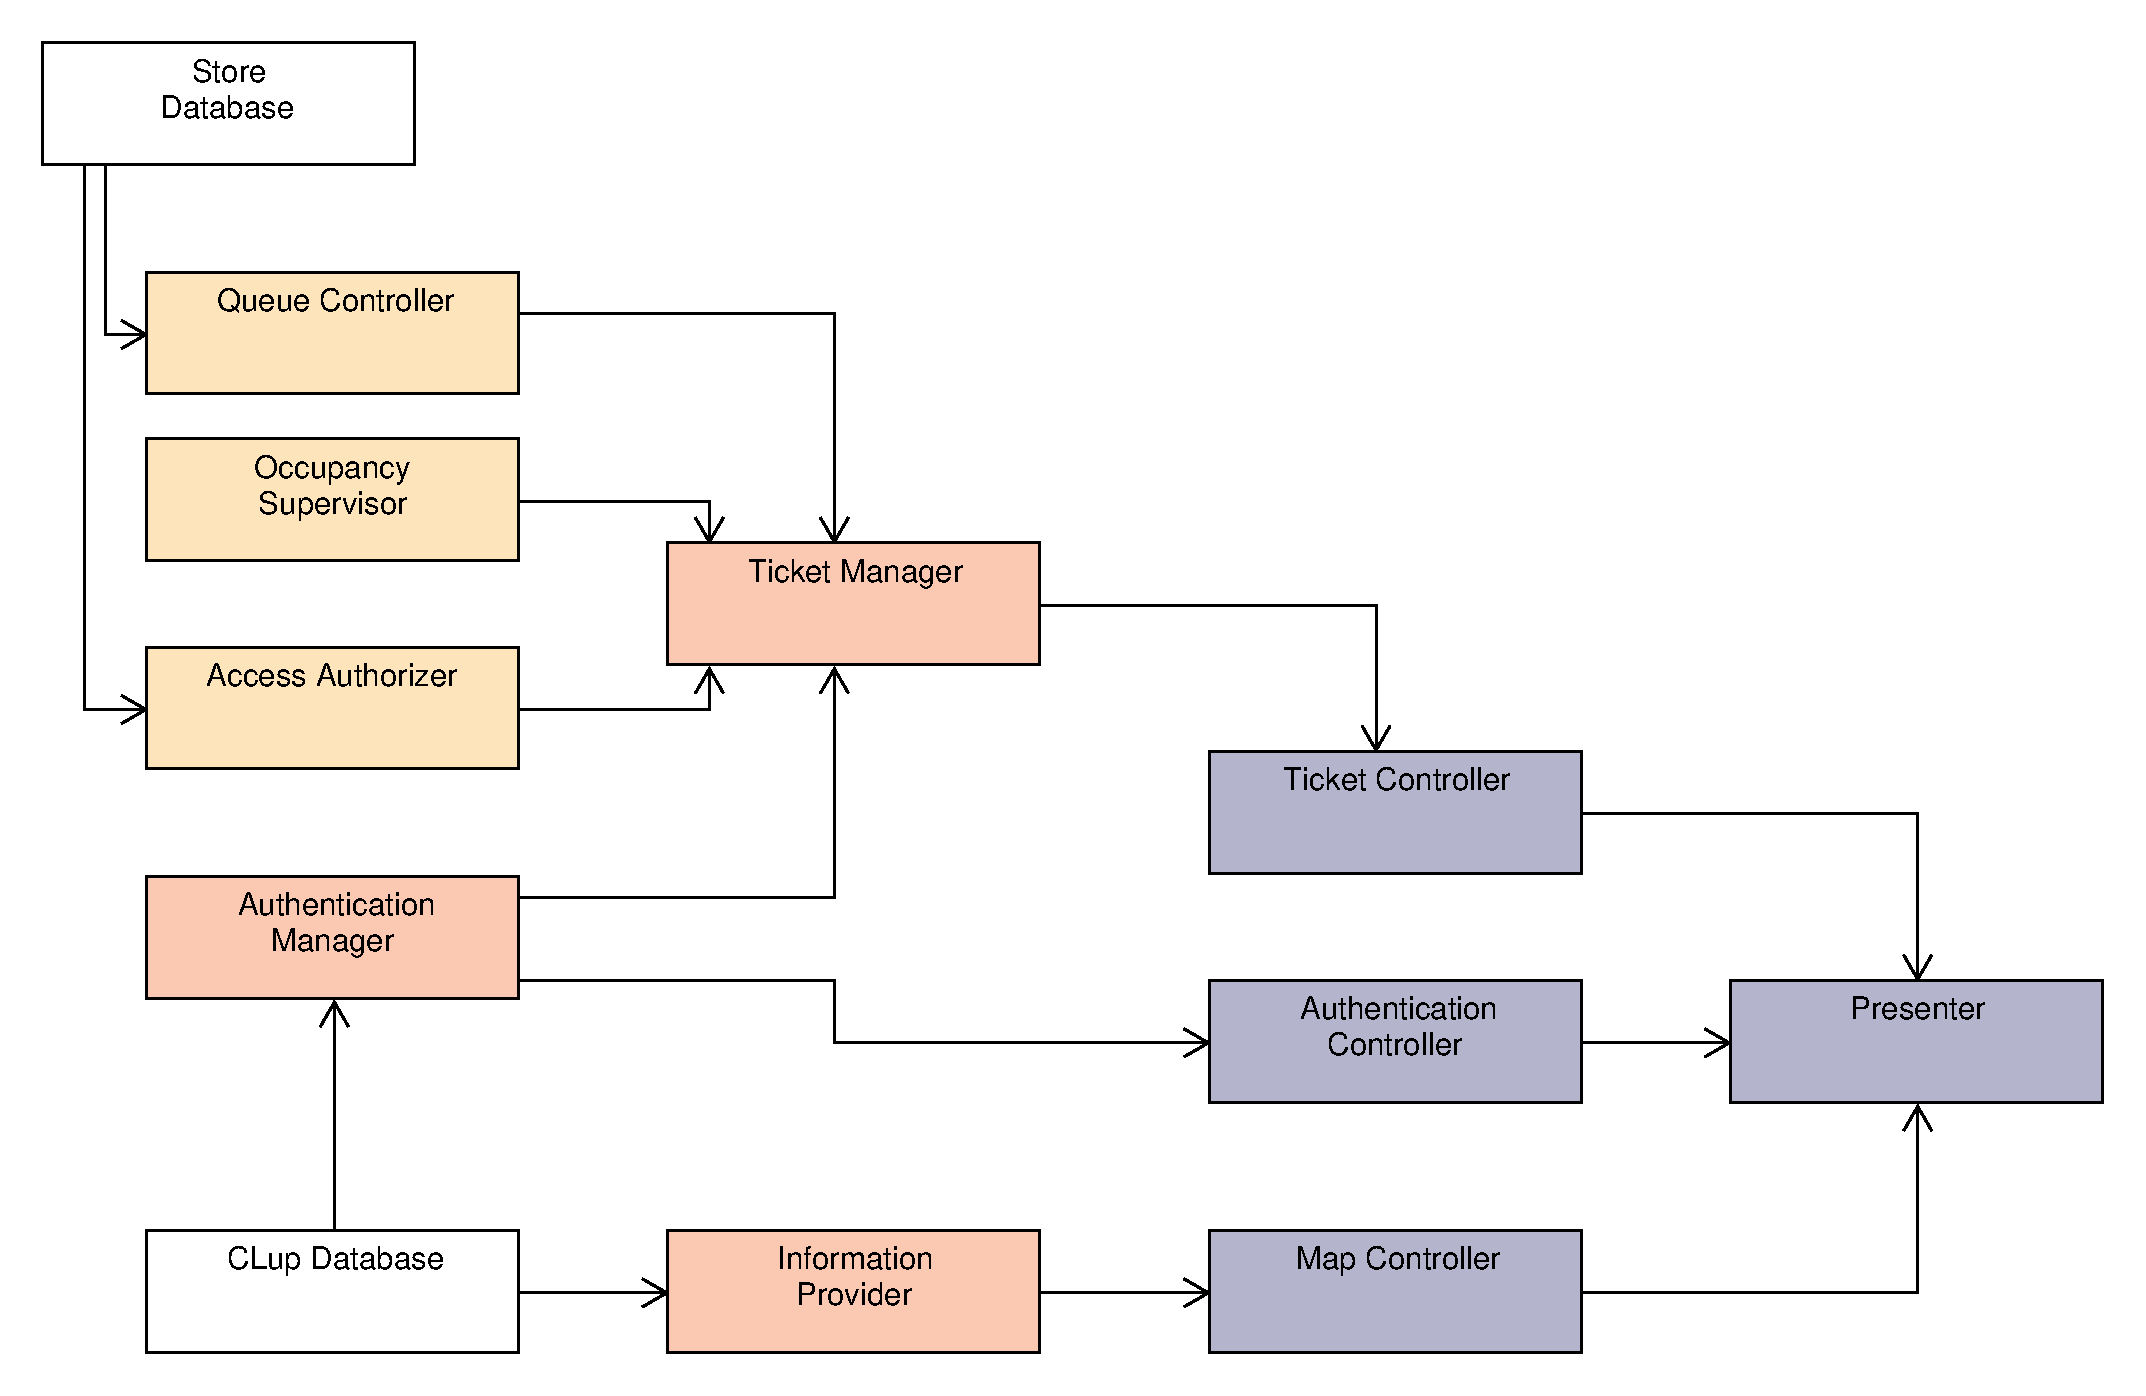
\includegraphics[width=\textwidth]{Images/Impl_Plan_1.pdf}
    \caption{\label{fig:UML_virtual_ticket_sequence}First Iteration of Implementation Plan}
\end{figure}

The first iteration sets up the system to provide the functionality for issuing a numbered ticket, either using the application or the ticket emitter. The first components to be set-up are the databases, then the development can continue with the essential backend components (CLup Server and Store System). After this, the development shifts on the frontend (CLup user application) essential features.

\clearpage

\subsubsection{Second Iteration}

\begin{figure}[H]
    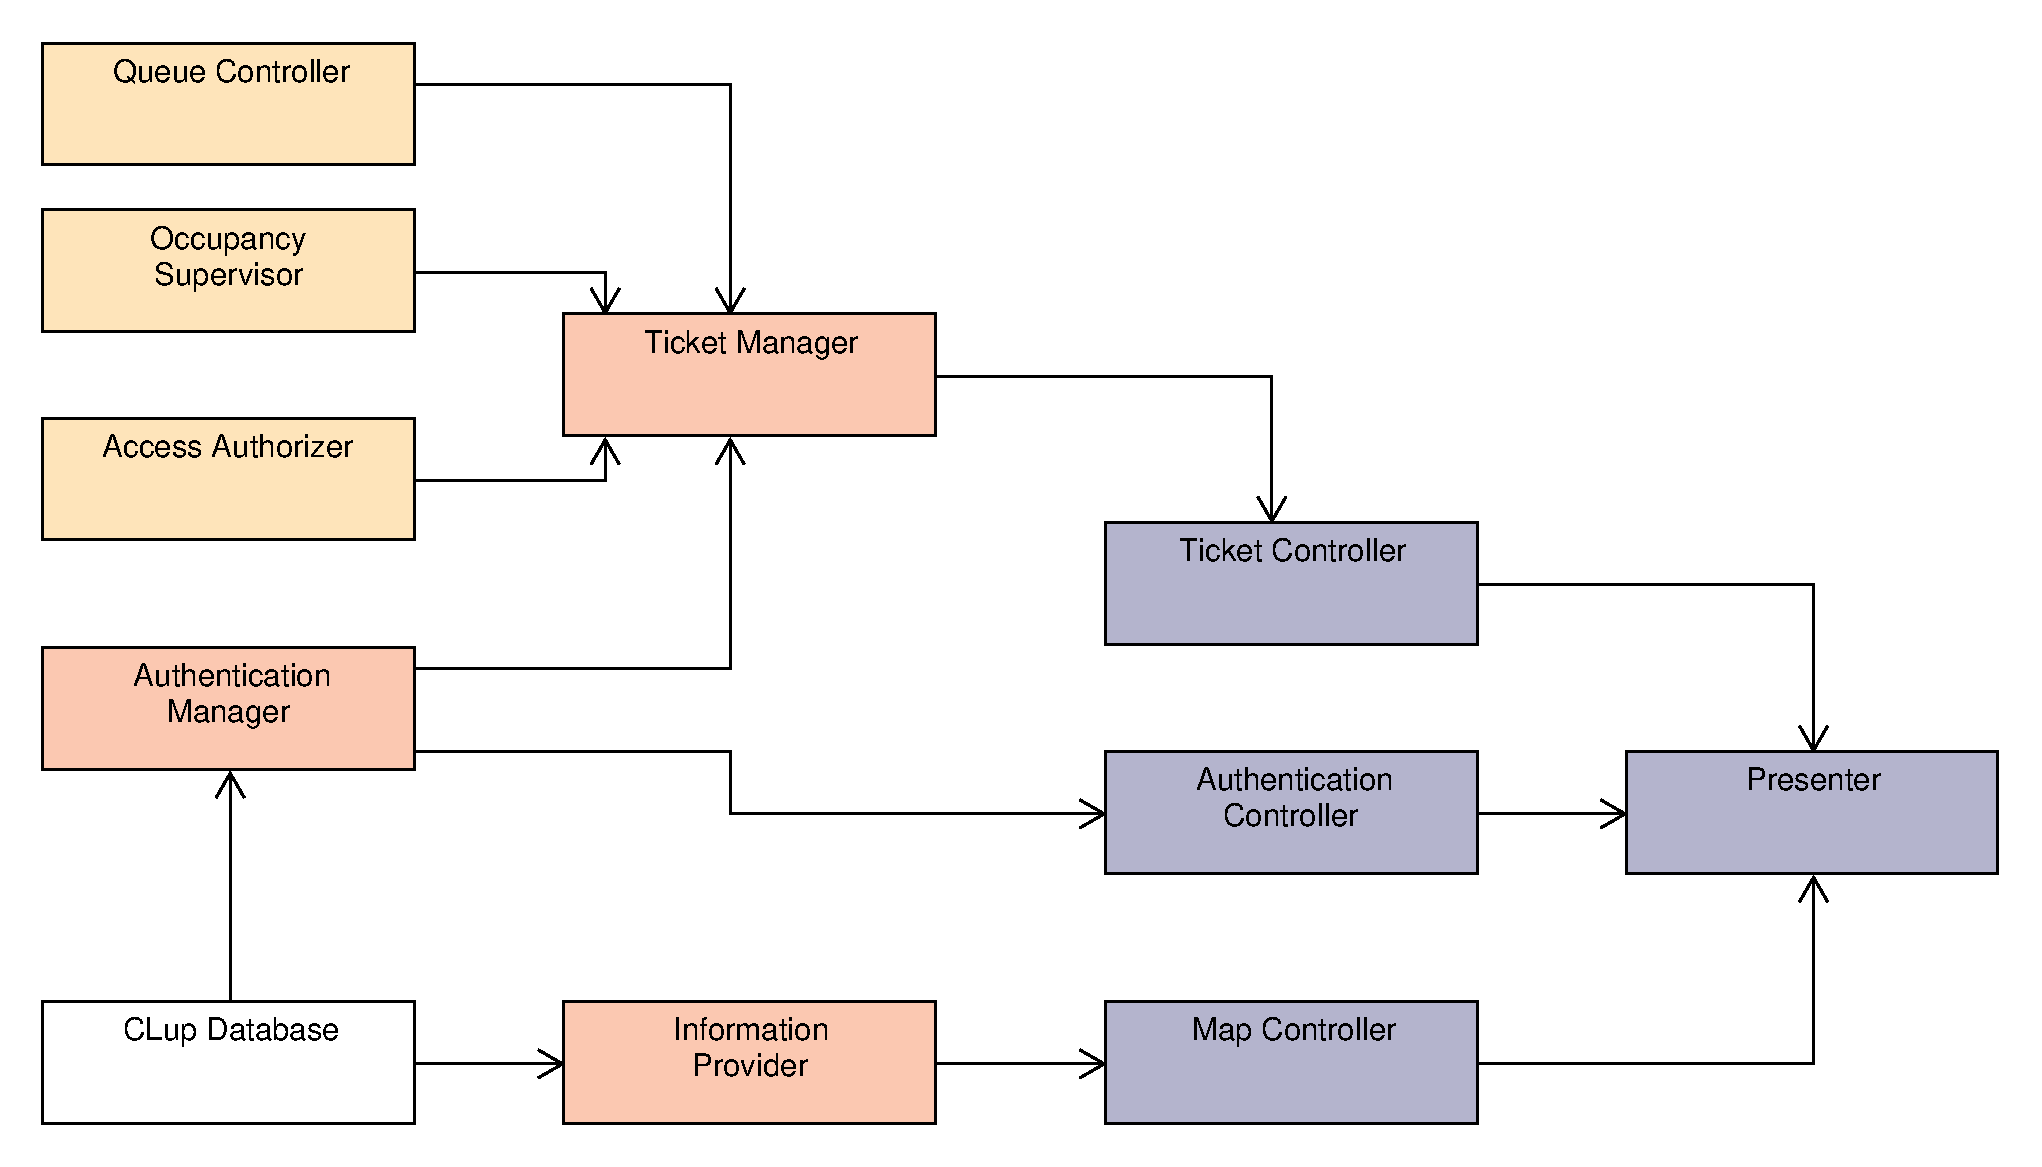
\includegraphics[width=\textwidth]{Images/Impl_Plan_2.pdf}
    \caption{\label{fig:UML_virtual_ticket_sequence}Second Iteration of Implementation Plan}
\end{figure}

In the second iteration the `Book a visit' feature is implemented. At first the required data structures are created in the CLup Database and the subsequent components are created (if they not exist yet) or expanded to host the new features.

\subsubsection{Third Iteration}
\begin{figure}[H]
    \centering
    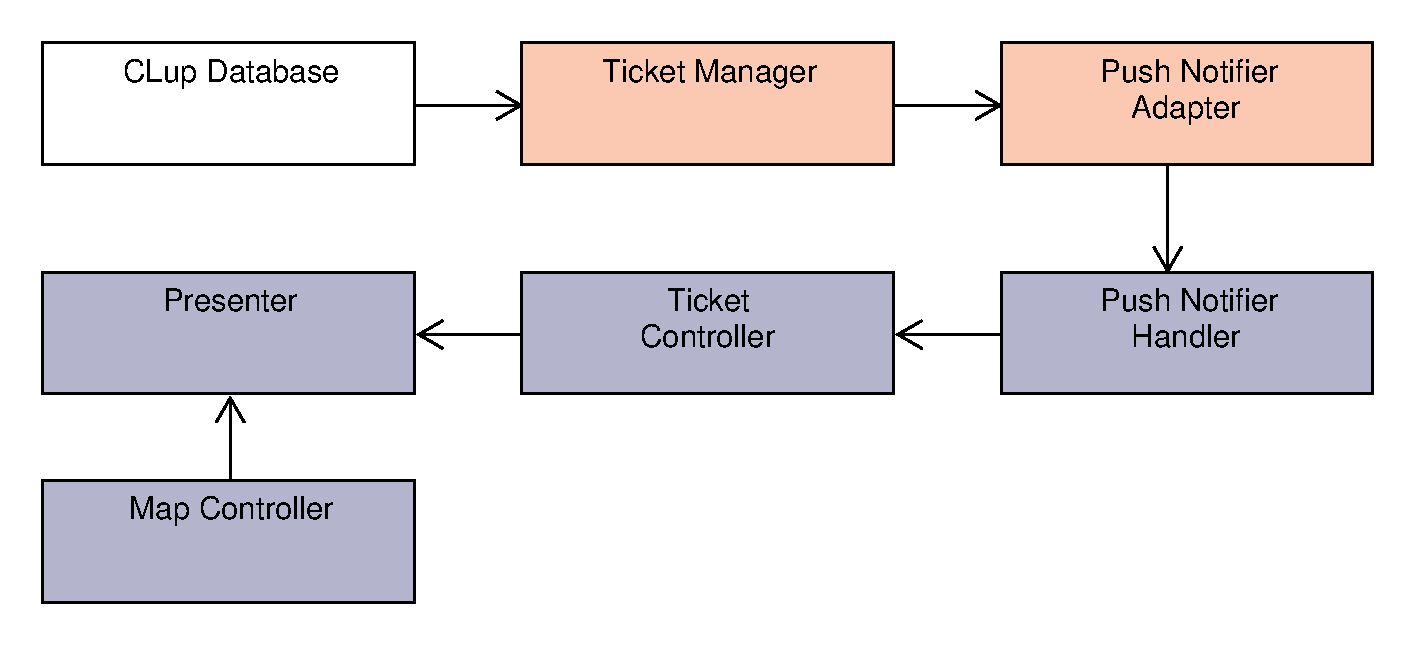
\includegraphics[width=0.8\textwidth]{Images/Impl_Plan_3.pdf}
    \caption{\label{fig:UML_virtual_ticket_sequence}Third Iteration of Implementation Plan}
\end{figure}

The last iteration adds nice to have features in the system like `push notifications' that require adding some new components and the `add store to favorites' which requires the expansion of the Map Controller and the Presenter components.

\subsection{Unit Testing}
Each component will be developed using mainly Test Driven Development (TDD) strategy. This strategy consist in writing the unit test cases before writing the application code, forcing the developer to use black box testing over white box testing. In this way the developer has to think at all combinations of the inputs before writing the code. When or after writing the code the developer can always add some white box test cases if they feel that this addition could improve the coverage and the effectiveness of the test cases.

The unit testing should not pose a constraint on the programming languages chosen to implement the system, because nowadays almost all mainstream languages provide a unit testing library (i.e. JUnit for Java).

\subsection{Integration and Testing}
The integration of the components can follow the implementation plan with its precedence relations. When a component is implemented and unit tested, the component can finally be integrated and tested with all the other previously developed components.

To start a new iteration, the integration test has to be passed in the previous iteration.

The integration test can start in parallel to the implementation of the components, in fact a Quality Assessment team can start to integrate and test a component together with its predecessors when its implementation is concluded.

\subsection{Other Development Tools}
To develop the S2B a \textbf{versioning system}, like git, must be used. This allows to keep the history of the implementation in a repository, track issues in an easier way, revert changes that created errors and share code between the developers in a straightforward way.

To add a change in the repository the developers perform `commits'; these commits include a message that explains briefly what are the contents of the commit. It's preferable to use a convention in these messages, to allow a program to automatically generate changelogs, and to force the developers to create small commits with small changes, instead of using big and monolithic commits that are difficult to understand. A widely used standard for commit messages is the \textbf{Conventional Commits}\footnote{https://www.conventionalcommits.org/en/v1.0.0/} Standard.

Another useful set of tools are \textbf{Continuous Integration (CI)} frameworks. These frameworks allow the developers to automate testing when pushing to a versioning system repository, which saves time and motivates developers to push code only when it passes all unit tests. CI works really well with a Test Driven Development Strategy.